\begin{example}
    \begin{figure}
        \centering
        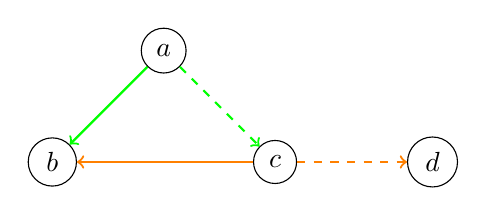
\begin{tikzpicture}[
                node distance={20mm},
                main/.style = {draw, circle},
                s/.style = {->,thick},
                d/.style = {->,thick,dashed} ]
            \node[main] (b) {$b$};
            \node[main] (a) [above right of=b] {$a$};
            \node[main] (c) [below right of=a] {$c$};
            \node[main] (d) [right of=c] {$d$};
            \draw[thick,green,->] (a) -- (b);
            \draw[thick,green,->,dashed] (a) -- (c);
            \draw[thick,orange,->] (c) -- (b);
            \draw[thick,orange,->,dashed] (c) -- (d);
        \end{tikzpicture}
        \caption{}
        \label{fig:blacklist}
    \end{figure}
    \begin{figure}
        \centering
        \begin{tikzpicture}
            \crd{0}{0}{$\emptyset$}
            \crd[left]{-2}{1}{$\s{p_1}$}
            \crd[left]{-2}{2}{$\s{p_1,q_1}$}
            \crd[left]{-2}{3}{$\s{p_1,q_1,ad_1}$}
            \crd[right]{2}{1}{$\s{q_2}$}
            \crd[right]{2}{2}{$\s{p_2,q_2}$}
            \crd[right]{2}{3}{$\s{p_2,q_2,ad_2}$}
            \draw [ultra thick] (-2,1) -- (-2,2);
            \draw [ultra thick] (-2,2) -- (-2,3);
            \draw [ultra thick] (0,0) -- (2,1);
            \draw [ultra thick] (0,0) -- (-2,1);
            \draw [ultra thick] (2,1) -- (2,2);
            \draw [ultra thick] (2,1) -- (2,3);
        \end{tikzpicture}
        \caption{}
        \label{fig:blacklist:es}
    \end{figure}

Consider the network in the figure \ref{fig:blacklist}.
Assume that two updates, $p$ and $q$ happening in the network.
$p$ replaces the path $ab$ with $ac$ and $q$ replaces
the path $cb$ with $cd$.
We use the event structure shown in \ref{fig:blacklist:es}
to model this network.
We use $p_1,p_2,q_1,q_2$ for the update and 
$ad_1,ad_2$ for the event of forwarding a packet from $a$
to $d$.
For simplicity, we do not consider forwarding events 
other than $ad$.
Using our causal mode, we can prove that lack of conflict
between $p_1$ and $q_1$ is an actual cause of 
$\s{p_1,q_1,ad_1}$ being a configuration of the event structure.
\end{example}